%
%    F U K U D A
%


\documentclass[10pt,b5paper,papersize,dvipdfmx]{jsbook}
% 会誌は B5 サイズです

\usepackage{vuccaken}
\usepackage{vuccaken2019}
\usepackage{cases}    %追加ありがとうございます、nkymさん!

% スタイルファイルの読み込みや自作マクロは、
% 最終的には vuccaken2019.sty の中に書いてください。
% とりあえずはここに書いてもらって構いません。


\begin{document} % 以下本文

% - - - - - - - - - - - - - - - - - - - - - - - - %
\kaishititle%
  {磁気単極子の存在仮定下における電磁気学の考察}% title
  {理工学部物理科学科1回生}% 所属
  {福田大和}% name
% - - - - - - - - - - - - - - - - - - - - - - - - %

% \setcounter{tocdepth}{2} % 目次にどこまで表示するか
% \tableofcontents % 目次出力
% \clearpage % 改ページ

\section*{はじめに}
前半で電磁気学の概要をかなーーーーーーーーーーーり駆け足で説明し、後半では私個人の考えを展開していきます。前半の説明は私の説明しやすい順番で、私の理解が及ぶ範囲で説明しています。具体的には、多くの電磁気学の教科書はクーロンの法則などの、あまり電磁気学に触れたことのない方にも直感的に分かりやすい関係式から初めて、マクスウェル方程式を導き、云々、という展開が一般的かと思います。しかし、今回は初めに電磁気学全てを支配するマクスウェル方程式を提示し、種々の関係式を導くという順序です。この順序にした理由は二つあり、一つは私が前述したような一般的な説明に馴染めないということ。ありていに言うと、うまく説明できる自信がない為です。もう一つは、ここでの主題である磁気単極子についての議論をするときに、この順序で説明した方がすんなり受け入れていただけるのではと考えたからです。あらかじめ断っておきますが、間違っている可能性も十二分にあり得ますのでそのことに留意してお読みいただければ幸いです。

\section{前提知識}
まず、ここではベクトルは太字で書きます。例えば、Aというベクトルは$\mathbf{A}$と書き、$\vec{A}$とは書きません。

\section{電磁気学概説}
\subsection{マクスウェル方程式}
ようやく電磁気学です。兎にも角にも、まずはマクスウェル方程式を見て頂きましょう。
\subsubsection{〈積分形〉}
\begin{numcases}
{}
\label{Gauss}
\int_S \mathbf{E}\cdot \mathbf{n} dS = \frac{1}{\epsilon_o} \int_V \rho dV \\
\label{Faraday}
\oint_C \mathbf{E}\cdot d\mathbf{r} = -\frac{d}{dt}\int_S \mathbf{B}\cdot\mathbf{n} dS \\
\label{Gauss2}
\int_S \mathbf{B}\cdot \mathbf{n}dS = 0 \\
\label{Ampere}
c^2 \oint_C \mathbf{B}\cdot d\mathbf{r} = \frac{1}{\epsilon_o}\int_S \mathbf{j}\cdot \mathbf{n}dS + \frac{d}{dt}\int_S \mathbf{E}\cdot \mathbf{n}dS
\end{numcases}
以上の四つがマクスウェル方程式と呼ばれる、電磁気学全てを支配する方程式達です。尚、文字の意味は$\mathbf{E}:電場、\mathbf{B}:磁場、\mathbf{j}:流束、\mathbf{n}:法線ベクトル、C:任意の閉曲線、S:任意の閉曲面、V:任意の閉曲面Sに囲まれた体積、\rho :電荷密度、c:光速$です。各方程式にはそれぞれ名前があり、
\ref{Gauss}式はガウスの法則、\ref{Faraday}式はファラデーの法則、\ref{Gauss2}式は磁場に関するファラデーの法則、\ref{Anpere}式はアンペール-マクスウェルの法則と呼ばれています。\ref{Gauss}式と\ref{Faraday}式が電場、\ref{Gauss2}式と\ref{Ampere}式が磁場に関する法則となんとなく考えて頂ければ結構です。
\subsubsection{〈微分形〉}
次に、積分形で書かれた上のマクスウェル方程式を微分形に変形したいと思います。 \par
まずはガウスの法則から。\ref{Gauss}式の左辺をガウスの定理で変形してやって、
\begin{align}
\int_V \bigtriangledown\cdot\mathbf{E} dV = \frac{1}{\epsilon_o} \int_V \rho dV
\end{align}
$V$は任意の体積としているので、
\begin{align}
\bigtriangledown\cdot\mathbf{E} = \frac{\rho}{\epsilon_o}
\end{align}
これがガウスの法則の微分形になります。\par
続いて、ファラデーの法則。\ref{Faraday}の左辺にストークスの定理で変形してやって、
\begin{align}
\int_S (\bigtriangledown\times\mathbf{E})\cdot\mathbf{n} dS = -\frac{d}{dt}\int_S \mathbf{B}\cdot \mathbf{n} dS
\end{align}
閉曲面$S$は時間変化しないとして、
\begin{align}
\int_S (\bigtriangledown\times\mathbf{E})\cdot\mathbf{n} dS = -\int_S \frac{\partial\mathbf{B}}{\partial t}\cdot \mathbf{n} dS
\end{align}
$S$は任意の閉曲面としているので、
\begin{align}
\bigtriangledown\times\mathbf{E} = -\frac{\partial\mathbf{B}}{\partial t}
\end{align}
これがファラデーの法則の微分形となります。
続いて、と行きたいところですが、磁場に関するガウスの法則とアンペール-マクスウェルの法則に」ついては、それぞれガウスの法則とファラデーの法則の変形と全く同じなので導出は割愛させていただきます。\footnote{最後のおまけに一応掲載。}結果だけ示すと、
\begin{align}
\bigtriangledown\cdot \mathbf{B} = 0\\
c^2 \bigtriangledown\cdot\mathbf{B} = \frac{\mathbf{j}}{\epsilon_o} + \frac{\partial\mathbf{E}}{\partial t}
\end{align}
以上より、マクスウェル方程式の微分形をまとめると、
\begin{numcases}
{}
\label{Gaussdif}
\bigtriangledown\cdot\mathbf{E} = \frac{\rho}{\epsilon_o}\\
\label{Faradaydif}
\bigtriangledown\times\mathbf{E} = -\frac{\partial\mathbf{B}}{\partial t}\\
\label{Gauss2dif}
\bigtriangledown\cdot \mathbf{B} = 0\\
\label{Amperedif}
c^2 \bigtriangledown\cdot\mathbf{B} = \frac{\mathbf{j}}{\epsilon_o} + \frac{\partial\mathbf{E}}{\partial t}
\end{numcases}
となります。
\subsection{静電場}
さて、ここからは前章で提示したマクスウェル方程式をガチャガチャいじって楽しんでいこうと思います。まずは静電場。ここで使うのは以下の2式です。
\begin{numcases}
{}
\label{Gauss1.2.2}
\int_S \mathbf{E}\cdot \mathbf{n} dS = \frac{1}{\epsilon_o} \int_V \rho dV \\
\label{Faraday1.2.2}
\oint_C \mathbf{E}\cdot d\mathbf{r} = 0
\end{numcases}
微分形だとこうなります。
\begin{numcases}
{}
\label{Gaussdif1.2.2}
\bigtriangledown\cdot\mathbf{E} = \frac{\rho}{\epsilon_o}\\
\label{Faradaydif1.2.2}
\bigtriangledown\times\mathbf{E} = 0
\end{numcases}
はい、先程提示したガウスの法則とファラデーの法則です。が、少し違いますよね?ファラデーの法則と\ref{Faraday1.2.2}式、\ref{Faradaydif1.2.2}式を見比べてみてください。右辺がどちらも0になっているのが分かるかと思います。これは静電場は時間変化しないから時間tで微分している項を0にしただけなのですが、この関係を{\bf 渦なしの法則}と呼びます。電場を閉曲線で線積分すると0になる、もしくは、電場の回転は0であると表現することもできます。これの何が重要なのか。それは保存力というものを考えると分かるかと思います。
\subsection{静磁場}
\subsection{時間変化}
\subsection{}

\section{オリジナル理論展開したい(願望)}
\subsection{なるようになーれー}

\section{おまけ}
\subsection{積分形→微分形}
\subsubsection{〈磁場に関するガウスの法則〉}

\subsubsection{〈アンペール-マクスウェルの法則〉}

\subsection{微分形→積分形}


\section{参考文献}
\renewcommand{\labelenumi}{[\arabic{enumi}]} % [1],[2],...
\begin{enumerate}
\item 小宮山 進・竹川 敦,『マクスウェル方程式から始める電磁気学』,裳華房,2016/9/15 第二版
\item (複数ある場合は追加)
\item @vuccaken, 物科研HP, \url{rp2017xy.starfree.jp}, 2019.
\end{enumerate}
\renewcommand{\labelenumi}{\arabic{enumi}.} % default

\end{document}


%\subsection{グラフや画像の挿入}
%\TeX はこれがめんどい。figure環境ごとコピペして使おう。
%
%\begin{figure}[htbp]
%  \centering
%  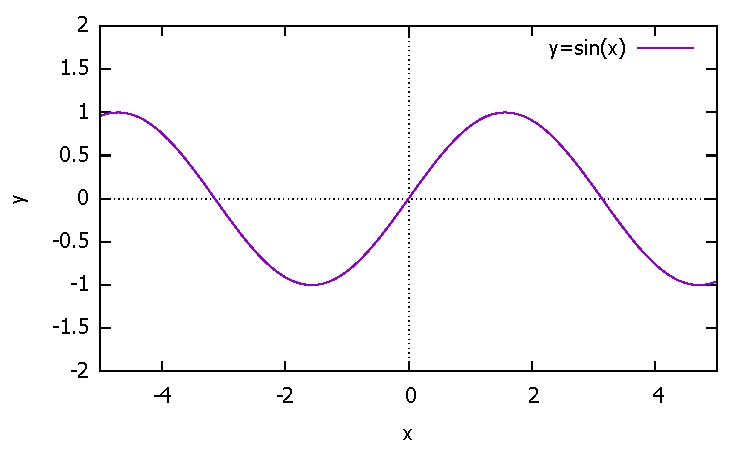
\includegraphics[width=10cm]{img/fig-sin.pdf}
%  \caption{$y=\sin x$のグラフ。gnuplotで作成した。}
%  \label{fig:sin}
%\end{figure}
%
%図\ref{fig:sin}より、sinが{\bfseries うねうね}であることがわかる。

%
%\subsection{ascmacパッケージ}
%枠で囲める。
%\begin{itembox}[l]{定義(ゼータ関数)}
%  $\Re(s) > 1$である任意の複素数$s$について、リーマンのゼータ関数$\zeta (s)$を以下のように定義する:
%  \begin{align*}
%    \zeta (s) := \sum_{n=1}^\infty \frac{1}{n^s}
%    \equiv \frac{1}{1^s} + \frac{1}{2^s} + \frac{1}{3^s} + \frac{1}{4^s} + \cdots
%  \end{align*}
%\end{itembox}

%
%\subsection{作図}
%\LaTeX と連携できるものとしては、picture環境やTi{\itshape k}ZやgnuplotやInkscapeなど色々な方法がありますが、ここではキーワードを挙げるに留めておきます。
%手描きを写真で撮ったり\footnote{明るさとコントラストをあげればそこそこキレイになる。}、パワポとかで作っても良いと思います\footnote{jpegは圧縮されて汚いので、pngか、ベクター形式のsvgとかpdfで作ると良い。}。

%
%\subsection{ソースコード}
%プログラムなどのソースコードを表示するにはlisting.styを使えばキレイに出力できますが、日本語に厳しい。そこで誰かが作ったplistings.styを代わりに使ってください。使い方はlisting.styと同じなので、そちらをキーワードにしてググってくだ
